\begin{figure}[htbp]
\section*{ TGFBR2}
\centering
\begin{subfigure}[b]{0.95\textwidth}
\centering
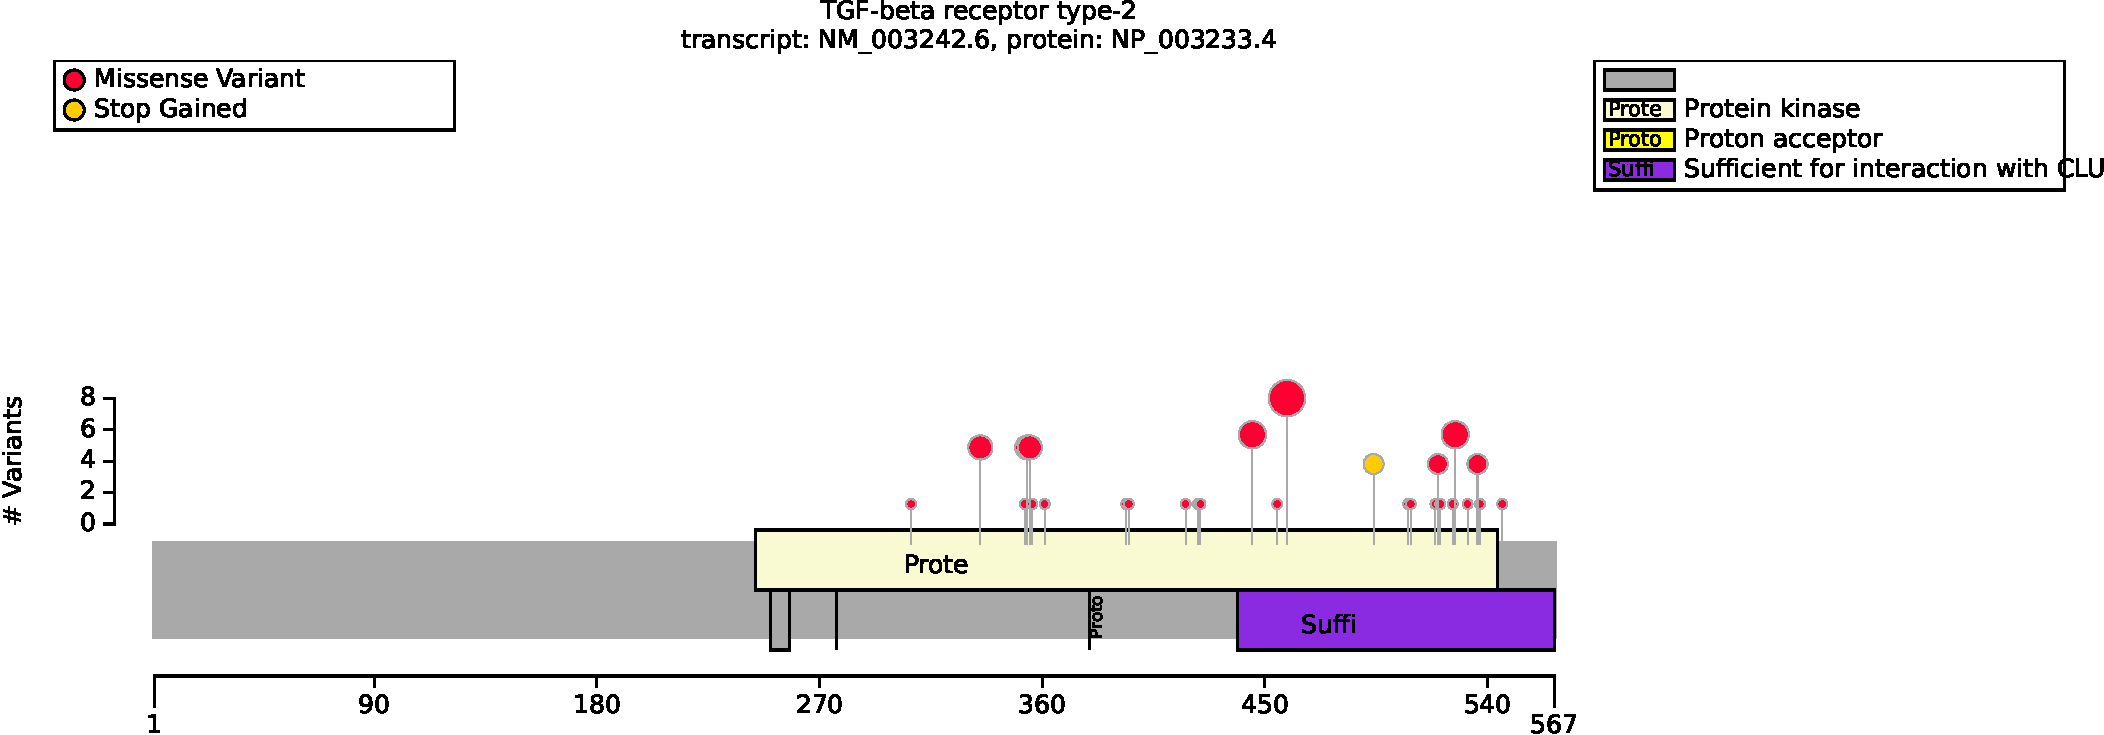
\includegraphics[width=\textwidth]{ img/TGFBR2_protein_diagram.pdf} 
\captionsetup{justification=raggedright,singlelinecheck=false}
\caption{Distribution of variants in TGFBR2}
\end{subfigure}

\vspace{2em}

\begin{subfigure}[b]{0.95\textwidth}
\centering
\resizebox{\textwidth}{!}{
\begin{tabular}{llllrr}
\toprule
Genotype (A) & Genotype (B) & total tests performed & significant results\\
\midrule
CLU interaction region & Other & 37 & 0\\
Missense & Other & 37 & 0\\
FEMALE & MALE & 35 & 0\\
\bottomrule
\end{tabular}
}
\captionsetup{justification=raggedright,singlelinecheck=false}
\caption{Fisher Exact Test performed to compare HPO annotation frequency with respect to genotypes.}
\end{subfigure}

\vspace{2em}

\caption{The cohort comprised 53 individuals (23 females, 30 males). 4 of these individuals were reported to be deceased. A total of 96 HPO terms were used to annotate the cohort. Disease diagnosis: Loeys-Dietz syndrome 2 (OMIM:610168). No statistically significant results identified. A total of 53 unique variant alleles were found in \textit{TGFBR2} (transcript: \texttt{NM\_003242.6}, protein id: \texttt{NP\_003233.4}).}
\end{figure}
